\documentclass[12pt,a4]{article}
\usepackage{amsmath,amsfonts,amsthm,amssymb, mathtools,steinmetz, gensymb, siunitx}	% LOADS USEFUL MATH STUFF
\usepackage{xcolor,graphicx}
\usepackage[left=1.5cm, top=2cm, right=1.5cm, bottom=2cm ,a4paper]{geometry} 				% ADJUSTS PAGE
\usepackage{setspace}
\usepackage{caption}
\usepackage{tikz}
\usepackage{pgf,tikz,pgfplots,wrapfig}
\usepackage{mathrsfs}
\usepackage{fancyhdr}
\usepackage{float}
\usepackage{array}
\usepackage{unicode-math}
\usepackage{booktabs}
\setmathfont{Libertinus Math}

\usetikzlibrary{decorations.text}
\pgfplotsset{compat=1.7}

\usetikzlibrary{decorations.pathreplacing,decorations.markings}
\usepgfplotslibrary{fillbetween}

\usepackage{hyperref}
\usepackage[style=ieee, maxbibnames=7]{biblatex}
\addbibresource{references.bib}


\AtBeginDocument{\hypersetup{pdfborder={0 0 0}}}

\title{
\includegraphics[scale = 0.5]{download.jpg}~ 
\\[1cm]
\textsc{Real Time Detection and Tracking of People in Crowds}
}
\author{\textsc{J L Gouws}
\\Supervisor: \textsc{Mr. J Connan}
\\ \emph{Computer Science Department, Rhodes University}}
\date{\today
\\[1cm]}



\usepackage{graphicx}
\usepackage{array}




\begin{document}
\fontencoding{T1}
\fontfamily{ppl}\selectfont
\thispagestyle{empty}

\maketitle

%In some sections you have to make a best guess (hypothesis), since you haven't done your MSc yet. 
\begin{abstract}
  Tracking objects in video streams is a powerful tool in computer vision.
  This research will investigate the recognition and tracking of multiple faces in settings where the faces are concurrently visible.
  The study will implement a tracking system that after, initialising with minimal input data, detects faces and tracks their motion in a video stream.
  The task of tracking starts by initialising the tracker with bounding boxes that define the faces of the targets in images. 
  %TODO fix these sentences
  The initialised tracker will be able to detect if a target face is present in or absent from an arbitrary video stream.
  The tracker will identify any visible target and follow its motion. 
  %TODO fix these sentences
  If a target face disappears and later reappears in the video stream, the tracker will be able to identify and track it again, provided the target remains in the field of view.
\end{abstract}

\newpage
\section{Introduction}
  Analysis of videos of crowds of people has many practical applications.
  Most real world situations that involve people have people that are moving.
  On top of that most often people are not isolated, but instead form groups of people.

  For these reasons it makes sense to investigate ways to develop a system that can efficiently and accurately detect and track multiple people in a video stream.
  Tracking targets in a video stream is by and large an understudied field.
  The literature is relatively limited in comparison with the number of real world applications of tracking systems.

\input{researchstatement}
\input{researchobjectives}
\section{Related Works}\label{sec:relatedWorks}
In 2011 \citeauthor{Kalal2011} invented the Tracking, Learning and Detection(TLD) framework for the longterm tracking of objects in a video stream.
Kalal's original implementation uses a median flow tracker, P-N learning, and a random forrest and nearest neighbour based detector \cite{KalalPHD}.
These three components give the respective tracking, learning and detection components of the system.

The learning compenent of TLD forms the backbone of the system, governing the interaction between the detector and tracker.
The three components exchange information as shown in Figure~\ref{fig:tld}, this allows the tracker to improve it's performance as time progresses \cite{Kalal2011}.
For the system to operate, it requires online learning--learning as data becomes available. 
Kalal developed the P-N Learning paradigm \cite{PNLearning}, a semi-supervised bootstrapping model \cite{murphy2012}, tailored to the needs of TLD.

\begin{figure}[!ht]
  \centering
   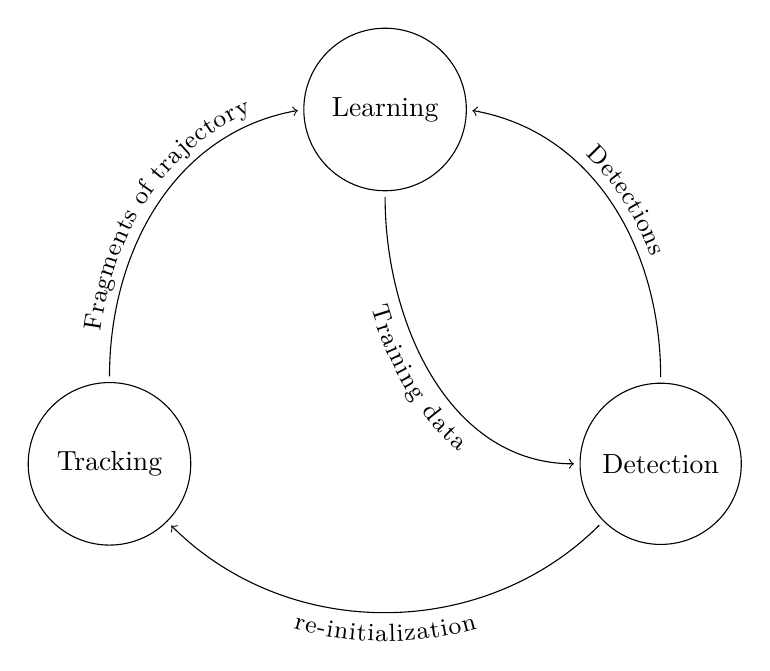
\begin{tikzpicture}[approach/.style={draw,very thick, fill=white, text width=5em,
         text centered, minimum height=2em,rounded corners=3ex, scale=0.1, everynode/.style={scale=0.1}},
         idea/.style={draw=black, circle,text width=5em,
            text centered, minimum height=2.5em},
         connections/.style={->,draw=black,shorten <=2pt,shorten >=2pt},
         reverseConnections/.style={<-,draw=black,shorten <=2pt,shorten >=2pt},
      ]

      \node[draw] at (0,0) (tracking) [idea]  {Tracking};
      \node[draw] at (3.5,4.5) (learning) [idea]  {Learning};
      \draw[connections, postaction={decorate, decoration={raise=1ex, text along path, text align=center, text={|\small|Fragments of trajectory}}}] (tracking.north)to[out=90,in=190] (learning.west) ;
      \node[draw] at (7,0) (detection) [idea]  {Detection};
      \draw[connections, postaction={decorate, decoration={raise=-2.5ex, text along path, text align=center, text={|\small|Training data}}}] (learning.south) to[out=270,in=180] (detection.west) ;
      \draw[reverseConnections, postaction={decorate, decoration={raise=1ex, text along path, text align=center, text={|\small|Detections}}}] (learning.east) to[out=350,in=90] (detection.north) ;
      \draw[reverseConnections, postaction={decorate, decoration={raise=-2.5ex, text along path, text align=center, text={|\small|re-initialization}}}] (tracking.south east) to[out=-45,in=225] (detection.south west) ;
   \end{tikzpicture}
   \caption{The interaction between tracking, learning and detection in TLD. Figure from \cite{Kalal2011}}
   \label{fig:tld}
\end{figure}

\citeauthor{Enriques2014} \cite{Enriques2014} propose Kernelized Correlation Filters(KCF) and the novel Dual Correlaion filter(DCF).
Both KCF and DCF use circulant matrices and the kernel Trick.
The implementation of KCF by \citeauthor{Enriques2014} uses a Gaussian Kernel, whereas the DCF implementation uses a linear kernel.
The calculations involved with the linear kernel are less computationally complex than KCF. 
DCF can, hence, be processed faster, but, at the cost of some tracking precision.

Work by \citeauthor{multichannelCorrFilters} \cite{multichannelCorrFilters} allows KCF and DCF to be applied to modern and useful feature descriptors.
\citeauthor{Enriques2014} show that KCF and DCF be be applied to Histogram of Oriented Gradient(HOG) features to track and detect objects in a video stream with lower computation times and better accuracy.
KCF and DCF applied to HOG features are shown to outperfrom many tracking systems Table~\ref{tab:trackers}.
The results shown by Table~\ref{tab:trackers} are obtained from running the algorithms on a standard four core desktop processor from \citedate{Enriques2014}.

\begin{table}
  \centering
  \begin{tabular}[t]{cccc}
    \toprule
    Algorithm & feature & Mean precision & Mean FPS \\
    \midrule
    KCF       & HOG     & 73.2\%         & 172      \\
    \hline
    DCF       & HOG     & 72.8\%         & 292      \\
    \hline
    KCF       & Raw pixels & 56.0\%      & 154      \\
    \hline
    DCF       & Raw pixels & 45.1\%      & 278      \\
    \midrule
    \midrule
    \multicolumn{2}{c}{TLD}   & 60.8\%      &  28      \\
    \hline
    \multicolumn{2}{c}{Struck\cite{struck}}& 65.6\%     &  20     \\
    \hline
    \multicolumn{2}{c}{MOSSE\cite{mosse}}& 43.1\%      &  615     \\
    \bottomrule
  \end{tabular}
  \caption{Comparison of various trackers, adapted from \cite{Enriques2014}}
  \label{tab:trackers}
\end{table}

The system implemented by \citeauthor{Enriques2014} does not, however, encorporate a failure recovery mechanism--section 8 of \cite{Enriques2014}.
In other words \citeauthor{Enriques2014} only explore KCF in the domain of ST.
This is in contrast to the original TLD system which provides a failure recovery mechanism in the detection component \cite{Kalal2011}.
The ST using KCF and DCF done by \citeauthor{Enriques2014} can be used in a TLD framework for LT.

\citeauthor{Ma2015Correlation} \cite{Ma2015Correlation} investigate the problem of single object LT using correlation tracking.
\citeauthor{Ma2015Correlation} use two Gaussian ridge regression \cite{murphy2012} models for tracking.
One model uses the relative change in background and target as time progresses, the other model tracks by using the target's appearance.
The first model is used to track the object's trajectory through fast motion and occlusions, and the second is used for scale change.
Using both tracking models they train an online detector that is both flexible(from first tracker model) and stable(from second tracker model).

\citeauthor{Ma2015Correlation} train a random fern classifier \cite{ferns2007} \cite{Kalal2011} online in order to handle tracker failure.
This solves the LT problem in a similar way to \citeauthor{KalalPHD}.

The Visual Object Tracking Challenge(VOT) is a challenge that benchmarks various trackers every year \cite{VOT2017} \cite{VOT2020}.
VOT investigates both ST and LT.
In recent years, VOT has also introduced a real time challenge \cite{VOT2020}.

There has also been investigation into the use of Convolutional Neural Networks in tracking \cite{CNNTracking}.
The work by \citeauthor{CNNTracking} offers high performance tracking of generic objects.
The system implemented by \citeauthor{CNNTracking} requires a large amount of offline training.

\citeauthor{onlineRL} \cite{onlineRL} propose a new online reinforcement learning method that can be used to train models with minimal input data.
\citeauthor{onlineRL} describe the \textit{Reanalyse} algorithm.
Given a state of a machine learning model the \textit{Reanalyse} algorithm generates training targets for the model from some input data.
When the model has improved by training, the \textit{Reanalyse} algorithm generates more training targets based on the new state of the model, the already seen input data, and any new input data.
The algorithm allows the available training data to be cycled--this allows the algorithm to extract most of the information from a limited dataset.

\section{Approach to Research}
  Initially I will start by reading literature on tracking and facial recognition.
  This will mainly start by reviewing Kalal's work in TLD, namely his Doctoral thesis \cite{KalalPHD}.

  Next I will go into a phase of re-implementing predator in C++, with help from the OpenCV libraries.
  Once this is stable and running with decent performance, I will move onto the next stage.

  Next I will be looking at ways to improve my implementation of the TLD system.
  I will mainly focus on looking at improving the tracking and detection stages of the system.
  I will then spend a small amount of time looking at the learning component, but do not intend to completely change it.

  Next I will extend the tracking and detection system so that it is able to identify and track multiple targets in a video stream.
  This will probably require a lot of work and testing.
  It is important that the system is both reasonably accurate.
  It is particularly that the system does not get confused and misidentify objects in the start up phase.
  There is always high potential for confusion in the start up of system, where there are potentially similar looking faces.

  Finally I will be looking at ways to enhance the performance of tracking multiple objects.
  This will come later and mainly be considered and extension.
  It would be useful to have the system run on mobile devices or micro-computers, with the potential to be extended to a distributed system.

\subsection{Timeline}
The timeline for this project has been revised since the Proposal version.
Most of the implementation deadlines now fall in the June and July Holiday, this is on account of exams and busy term times.
\begin{center}
  \begin{tabular}{l l}
    \toprule
      Time & Deliverable\\
    \midrule
      30 March 2022     & Seminar 1: Presentation of project\\
      11 April 2022     & Draft proposal\\
      19 April 2022     & Final proposal\\
      6 May 2022        & Literature review\\
      20 May 2022       & Obtaining suitable public videos\\
      28 May 2022       & Functional re-implementation of TLD\\
      28 June 2022      & Using KCF as Tracking stage of tracker\\
      30 June 2022      & Implementing DCF and comparing to KCF\\
      6 July 2022       & Reviewing VOT for better trackers\\
      11 July 2022      & Investingating random fern detectors\\
      11-13 July 2022   & Seminar 2: Progress Presentation\\
      25 July 2022      & Final decision on Tracking and Detection stages.\\
      12 August 2022    & Extension of system to multiple targets\\
      19 August 2022    & Progress Report\\
      26 August 2022    & Test and make small improvements the system\\
      3 October 2022    & First Draft of thesis\\
      10 Octorber 2022  & Completion of implementation\\
      14 October 2022   & Short ACM-style paper\\
      17-19 October 2022& Seminar 3: Final Oral presentation\\
      28 October 2022   & Final project submission\\
    \bottomrule
  \end{tabular}
\end{center}

\section{Limitations}
  The first concern of this research is in regards to ethics.
  Owing to ethical concerns, the system can only be tested on public data, which limits the test cases for the system.
  An ethical clearance is required to test the system on examples that are closer to real world applications.
  Time restrictions on the project make doing an ethical clearance impractical.

  Further on this point, the second limitation of this research is time.
  The project is set to take one year, being an honours project.
  There is only so much literature that can be reviewed and still allow for the implementation of a system.
  On account of this restiction, the research might not explore certain areas of concern.

  This research is only concerned with the tracking of faces.
  There are many other features that can be used to detect and track humans, for example gait. 
  Sometimes, there are also needs to track objects other than faces. 
  The system implemented by the research cannot guarantee tracking capabilities of objects other than human faces.

  There will be an upper limit on the number of faces that can be tracked simultaneously in real time.
  There are two problematic cases: First, limited compute power, second screen space.
  The first case occurs if the runtime complexity of the implemented system increases proportionally to the number of faces being tracked.
  Formally, if system has runtime complexity worse than $O(1)$, the system will eventually fail to track, in real time, as more faces are added.
  The second problem case occurs in very large, dense crowds of faces where there is not enough space in the field of view for all the faces, or some faces are captured in insufficient resolution.

\section{Applications}
  This reaseach has multiple real world applications.
  One includes an automated class register that can be used in schools or for university lecture attendance.

  Another application on the larger scale is a security system for monitoring the motion of people.
  This application requires the system to be extended to a distributed system.
  This could enhance airport security for example, adding functionality to label suspected terrorists.

  The system also has potential to be used as an assistive technology for visually impaired people.
  If the system can be ported to a mobile device, it could help a visually impaired person identify people at a party or on a television program.
  This application assumes the system has had the appropriate offline training in it's initialization phase.


\printbibliography

\end{document}
